\chapter{Gamma-Ray Astronomy}
\label{ch:gamma-ray-astronomy}

In recent years, gamma-ray astronomy has become an important research field in astroparticle physics.
The term gamma-rays is generally denoted as photons with energies above \SI{100}{\kilo\eV}
\cite{funk}. Due to this high-energy nature, gamma rays pose some of the most powerful \gls{cr} in
the universe and since they travel in straight lines, it is possible to pinpoint their sources accurately.

For the past two decades, ground-based \gls{iact} experiments like the \gls{magic} telescopes, the \gls{veritas} and
the \gls{hess} have been monitoring these \gls{vhegr} to gain an understanding of their production.


\begin{figure}[h]
    \centering
    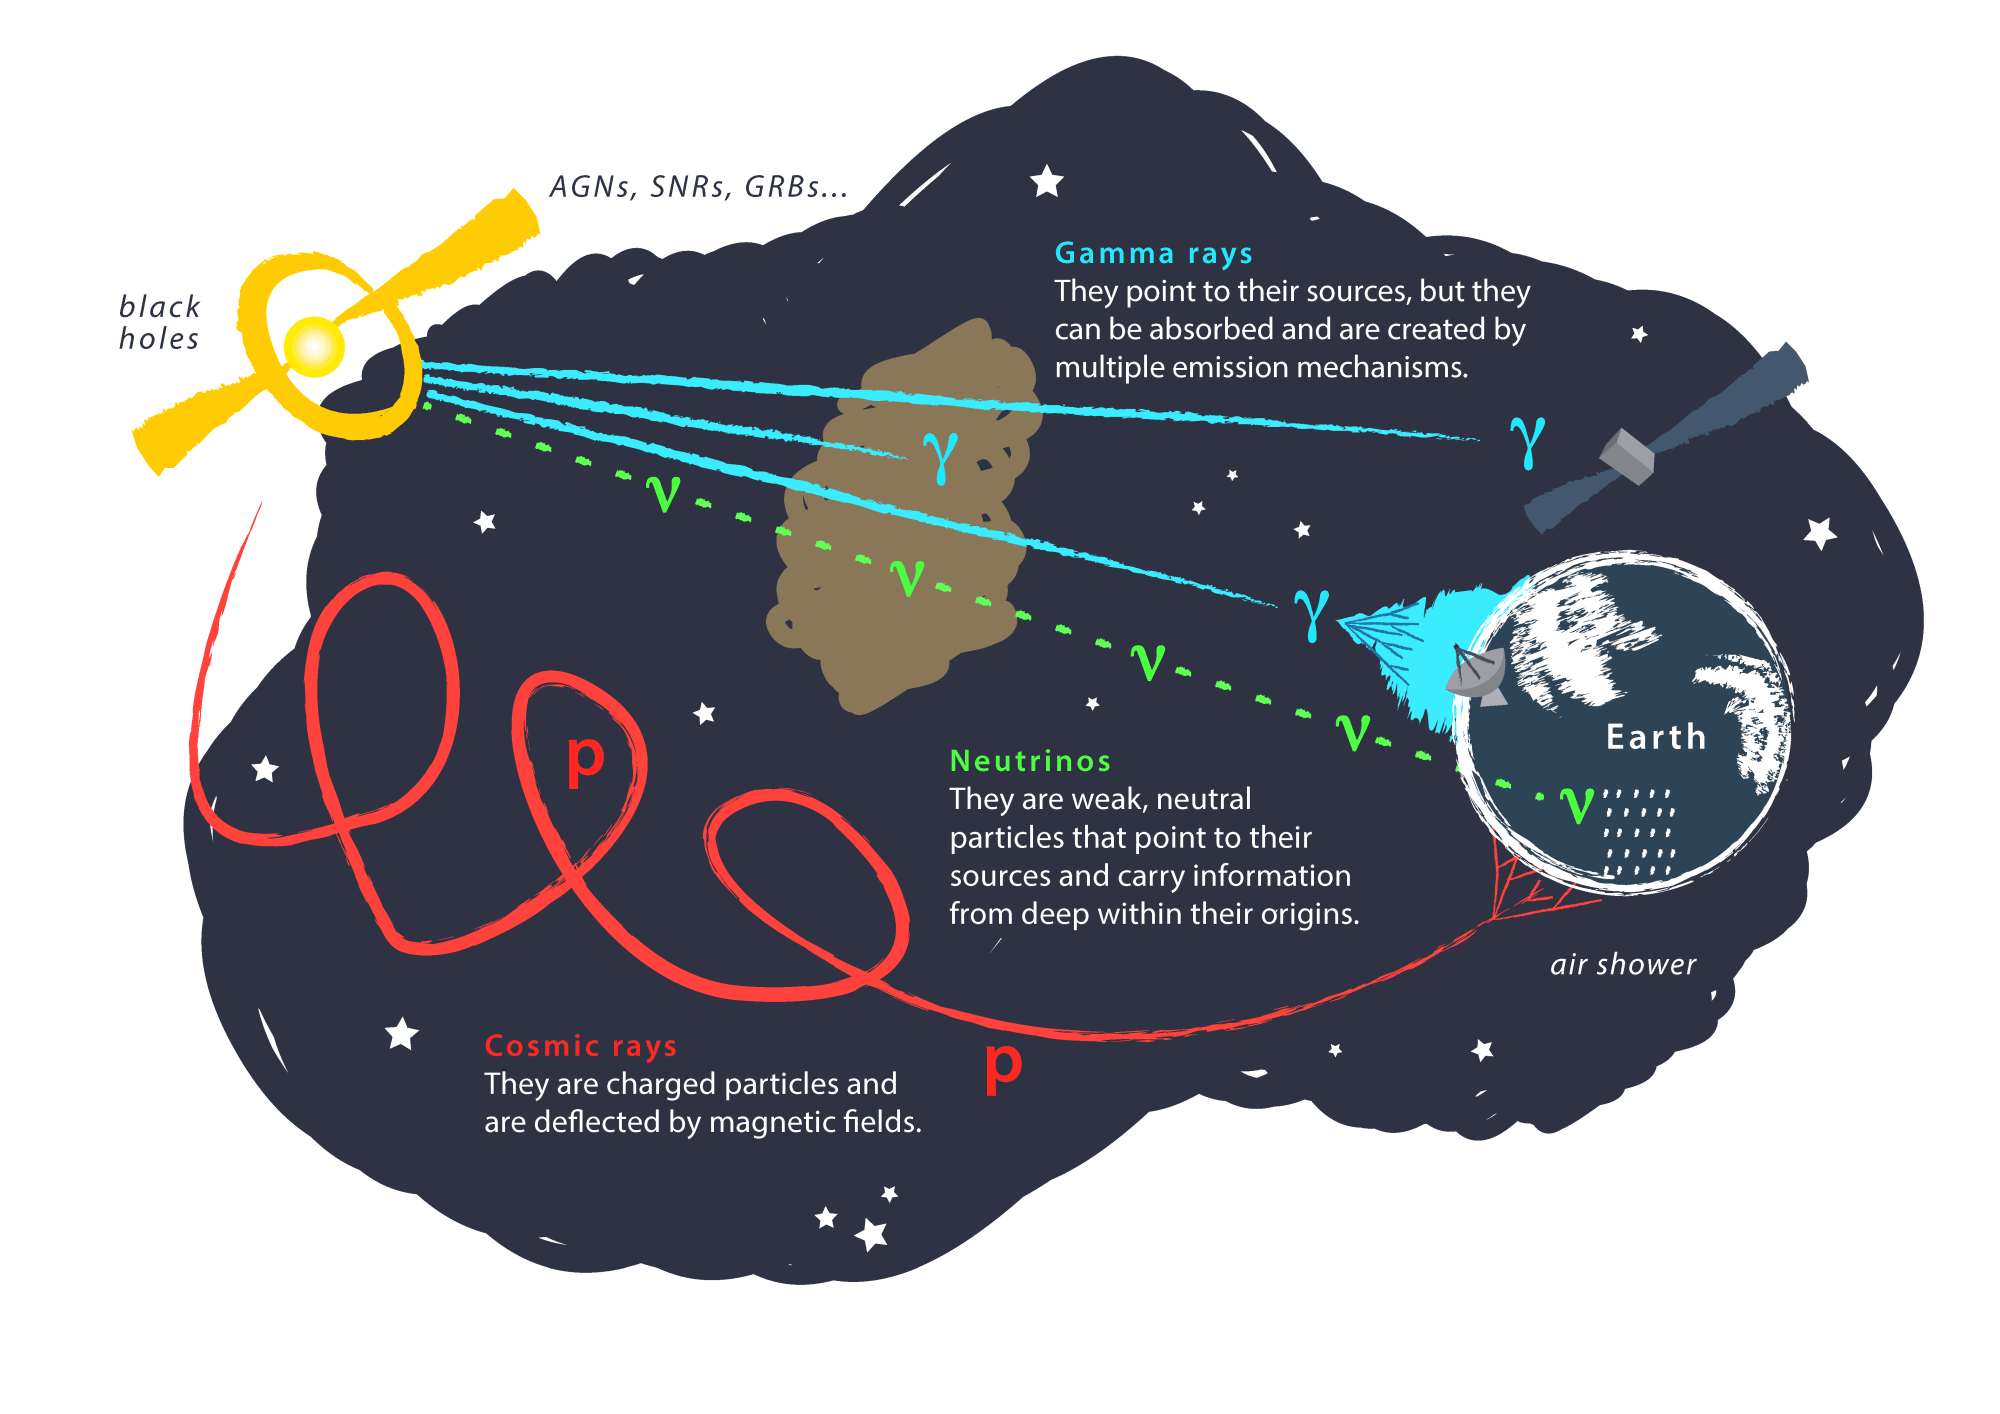
\includegraphics[width=0.8\textwidth]{graphics/figure5.png}
    \caption{Different types of cosmic rays on their way to Earth. Charged particles like protons and electrons
    are deflected by magnetic fields and therefore making it hard to pinpoint the source. Only the
    origin of photons and neutrinos can be reconstructed directly since they are uncharged particles
    and therefore travel in straight lines. However, photons can be absorbed or created in multiple
    mechanisms. Since neutrinos only rarely interact with matter via the weak force, their detection
    is significantly harder than for photons \cite{fig5}.}
    \label{fig:fig5}
\end{figure}

